\documentclass[letterpaper,12pt]{article}
\usepackage{amsmath,amsfonts,amsthm,amssymb,graphicx,mathtools,tikz,hyperref}
\usepackage{esvect,esint, subcaption, mathrsfs,comment, quiver, faktor}
\usepackage[onehalfspacing]{setspace}
\usepackage[ddmmyyyy]{datetime}
\renewcommand{\dateseparator}{.}


% place figures and tables where it seems like they should be
\usepackage{float}
\floatplacement{figure}{H}
\floatplacement{table}{H}

% automatically center figures/tables
\makeatletter
\g@addto@macro\@floatboxreset{\centering}
\makeatother

\usepackage{tocvsec2}
\usepackage[bookmarksdepth=subsection]{hyperref}
\usepackage{bookmark}
\usepackage[margin=1in]{geometry}
\usepackage{authblk}
\usepackage{titling}
\setlength{\droptitle}{-1in}

\input{Library/Fonts/BlackboardBold.tex}
\input{Library/Fonts/MathCalligraphy.tex}

\renewcommand\qedsymbol{$\blacksquare$}
\renewcommand{\bar}[1]{\overline{#1}}
\renewcommand{\epsilon}{\varepsilon}

\newcommand{\ita}[1]{\textit{#1}}
\newcommand{\com}[2]{#1\backslash#2}
\newcommand{\oneton}{\{1,2,3,...,n\}}
\newcommand\idea[1]{\begin{gather*}#1\end{gather*}}
\newcommand\ef{\ita{f} }
\newcommand\eff{\ita{f}}
\newcommand\proofs[1]{\begin{proof}#1\end{proof}}
\newcommand\inv[1]{#1^{-1}}
\newcommand\setb[1]{\{#1\}}
\newcommand\en{\ita{n }}
\newcommand{\vbrack}[1]{\langle #1\rangle}
\DeclareMathOperator{\rank}{rank}
\DeclareMathOperator{\ord}{ord}
\DeclareMathOperator{\Span}{span}
\DeclareMathOperator{\Int}{Int}
\DeclareMathOperator{\cl}{cl}
\DeclareMathOperator{\diam}{diam}

\theoremstyle{plain}
\newtheorem{theorem}{Theorem}
\newtheorem{axiom}{Axiom}
\newtheorem{lemma}[theorem]{Lemma}
\newtheorem{proposition}[theorem]{Proposition}
\newtheorem{postulate}{Postulate}
\newtheorem*{corollary}{Corollary}

\theoremstyle{definition}
\newtheorem*{definition}{Definition}
\newtheorem{conjecture}{Conjecture}
\newtheorem{example}{Example}

\newtheorem*{HW}{Homework}

\theoremstyle{remark}
\newtheorem*{remark}{Remark}
\newtheorem*{claim}{Claim}
\newtheorem*{note}{Note}

\pretitle{
    \begin{center}
        \fontsize{14pt}{1em}
        \bfseries\selectfont
            Prof. Claudio Landim \\
            https://www.youtube.com/playlist?list=PLo4jXE-LdDTQq8ZyA8F8reSQHej3F6RFX \\
            \vspace{14pt}
}

\posttitle{\end{center}}
\preauthor{\begin{center}\fontsize{12pt}{1em}\selectfont}
\postauthor{\end{center}}
\predate{\begin{center}\fontsize{12pt}{1em}\selectfont}
\postdate{\end{center}}

% section heading formatting
\renewcommand{\thesection}{\Roman{section}.}

\usepackage{sectsty}
\sectionfont{\centering\fontsize{12pt}{1em}\selectfont}

\title{Analysis I}

%%%%%%%%%%%%%%%%%%%%%%%%%%%%%%%%%%%%%%%%%%%%%%%%%%%%%%%%%%%%%%%%%%%%%%%%%%%%%%%%
% Your names go here (one should be underlined)
%%%%%%%%%%%%%%%%%%%%%%%%%%%%%%%%%%%%%%%%%%%%%%%%%%%%%%%%%%%%%%%%%%%%%%%%%%%%%%%%
\author{Alec Zabel-Mena}
\affil{Universidad de Puerto Rico, Recinto de Rio Piedras}

\begin{document}
\maketitle

\section*{Lecture 0: A Nonmeasurable Set}

Consider the following half-open bounded interval
\begin{figure}[h]
    \centering
    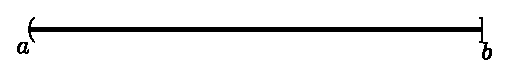
\includegraphics[scale=1.0]{Figures/half_open.eps}
    \caption{}
    \label{figure_1}
\end{figure}

Then the length of $(a,b]$ is $l((a,b])=b-a$. We can define the length of an
interval as a function $l:2^\R \xrightarrow{} \R^+_\infty$, where
$\R^+_\infty=\R^+ \cup \{\infty\}$. Notice then that the following hold for our
function $l$:
\begin{enumerate}
    \item[(1)] $l(A+y)=l(A)$, where $A+y=\{a+y : a \in A\}$.

    \item[(2)] If $A \subseteq B$, then  $l(A) \leq l(B)$.

    \item[(3)] For any collection $\{A_n\}$ of disjoint intervals, we have
        \begin{equation*}
            l(\bigcup{A_n})=\sum{l(A_n)}
        \end{equation*}
\end{enumerate}

Now, we wish to define a general function on all subsets of $\R$,  $\mu:2^\R
\xrightarrow{} \R^+_\infty$ such that
\begin{enumerate}
    \item[(1)] $\mu((a,b])=b-a$

    \item[(2)] If $A \subseteq B$, then  $\mu(A) \leq \mu(B)$.

    \item[(3)] $\mu(A+y)=\mu(A)$

    \item[(4)] For any disjoint collection of sets $\{A_n\}$,
        \begin{equation*}
            \mu(\bigcup{A_n})=\sum{\mu(A_n)}
        \end{equation*}
\end{enumerate}
We would also like $\mu(\emptyset)=0$.

\begin{theorem}\label{theorem_1}
    No such function $\mu:2^\R \xrightarrow{} \R^+_\infty$ satisfying (1)--(4)
    exists.
\end{theorem}
\begin{proof}
    Suppose such a function exists. Define the equivalence relation $\sim$ on
    $\R$ such that
    \begin{equation*}
        x \sim y \text{ if, and only if } x-y \in \Q
    \end{equation*}
    Let $\Lambda=\faktor{\R}{\sim}$. Then $\Lambda$ is not countable, as that
    would make $\R$ countable which is impossible. Now, let $R \subseteq [0,1]$
    a collections of representatives of equivalence classes of $\Lambda$, choose
    one representative for each element, by the axiom of choice, that is
    \begin{equation*}
    R=\{x : [x] \in \Lambda \text{ and } x=y \text{ if } [x]=[y]\}
    \end{equation*}
    Now, let $p,q \in \Q$, then we have that either  $R+p=R+q$ or that  $R+p$
    and  $R+q$ are disjoint. Suppose that they are not disjoint, and choose an
    $x \in (R+p) \cap (R+q)$. Then $x=\alpha+p$ and $x=\beta+q$. Thus
    $\alpha-\beta=q-p \in \Q$ which makes $\alpha \sim \beta$. By our
    definition, then  $\alpha=\beta$, and we get  $R+p=R+q$.

    Now consider the collection of all $\{R+q\}_{q \in \Q}$. This collection is
    disjoint as each $q$ is distinct, and consider
    \begin{equation*}
        \mu(\bigcup{R+q})=\sum{\mu(R+q)} \text{ for } -1<q<1
    \end{equation*}
    Notice that $\bigcup{R+q} \subseteq (-1,2)$, and so we get
    \begin{equation*}
        \sum{\mu(R+q)} \leq \mu((-1,2))=3 \text{ for } -1<q<1
    \end{equation*}
    By (3), we also get that
    \begin{equation*}
        \mu(R+q)=\mu(R)
    \end{equation*}
    so that
    \begin{equation*}
        \sum{\mu(R)} \leq \mu((-1,2))=3
    \end{equation*}
\end{proof}

Now, since this sum is bounded, $\mu(R)=0$. On the other hand, notice that
$(0,1) \subseteq \bigcup{R+q}$. So that $\mu((0,1))=1 \leq \mu(R)=0$. This is a
contradiction. Therefore no such $\mu$ exists.

\begin{definition}
    We call a set for which no such function $\mu$, satisfying (1)--(4) exists a
    \textbf{nonmeasurable set}.
\end{definition}

We would now like to restrict our sets to those that permit such a function
$\mu$ to exist; the so called ``measurable'' sets.

\section*{Lecture 1: Review}

We begin with a review of some prelimanary results of set theory and advanced
calculus.

\begin{definition}
    Let $A$ and $B$ be sets, and let $f:A \rightarrow B$ be a map of $A$ into
   $B$. We say that $f$ is  \textbf{1--1} if for every  $x,y \in X$,  $f(x)=f(y)$
   implies $x=y$. We say $f$ is \textbf{onto} if for every $y \in B$, there is
   an  $x \in A$ for which $y=f(x)$. We say that $f$ is a  \textbf{1--1
   correspondence} of $A$  \textbf{onto} $B$ if  $f$ is both 1--1 and onto and
   onto.
\end{definition}

\begin{theorem}[Beinstern's Theorem]\label{thm_1}
    Let $A$ and  $B$ be sets. If there is a 1--1 map of $A$ into  $B$, and a
    1--1 map of  $B$ into $A$, then there exists a 1--1 correspondence of
    $A$ onto  $B$.
\end{theorem}

\begin{axiom}[The Axiom of Choice]\label{axm_1}
    Suppose that $\{A_\alpha\}_{\alpha \in \Lambda}$ is a collection of nonmepty
    sets indexed by the set $\Lambda$. Then there exists a map $f:\Lambda
    \rightarrow \bigcup{A_\alpha}$ called a \textbf{choice function}, defined by
    the rule $f(\alpha) \in A_\alpha$ for all $\alpha \in \Lambda$.
\end{axiom}
\begin{remark}
    What this axiom says is that given any (not necesarrily countable)
    collection of sets, one can ``choose '' an element from each set.
\end{remark}

\begin{definition}
    We define an \textbf{order} on a set $A$ to be a relation  $<$ satisfying
    the following properties for all $a,b,c \in A$:.
    \begin{enumerate}
        \item[(1)] $a<a$  (Reflexive).

        \item[(2)] If $a<b$ and  $b<a$, then  $a=b$  (Antisymmetry).

        \item[(3)] If $a<b$ and  $b<c$, then  $a<c$  (Transitivity).
    \end{enumerate}
     We say that elements $a,b \in A$ are \textbf{comparable} under $<$ if
     either $a<b$ or $b<a$. If every element of $A$ is comparable, then  $<$ is
     called a  \textbf{total order}.
\end{definition}

\begin{definition}
    Let $A$ be a set with order  $<$. We call an element  $x \in A$ a
    \textbf{maximum} of $A$ if  $x<a$ implies  $x=a$ for all $a \in A$. If $B
    \subseteq A$, then we call an element $a \in A$ an \textbf{upper bound} of
    $B$ if  $b<a$ for all  $B$ in  $B$; and we say  $B$ is  \textbf{bounded
    above}. If $b<a'$ implies that  $a<a'$ for any  $a' \in A$, then we call
    $a$ a  \textbf{least upper bound} of $B$ and write  $\sup{B}=a$.
\end{definition}

\begin{definition}
    Let $A$ be a set with order  $<$. We call an element  $x \in A$ a
    \textbf{minimum} of $A$ if  $a<x$ implies  $x=a$ for all $a \in A$. If $B
    \subseteq A$, then we call an element $a \in A$ an \textbf{lower bound} of
    $B$ if  $a<b$ for all  $B$ in  $B$; and we say  $B$ is  \textbf{bounded
    below}. If $a'<b$ implies that  $a'<a$ for any  $a' \in A$, then we call
    $a$ a  \textbf{greatest lower bound} of $B$ and write  $\inf{B}=a$.
\end{definition}

\begin{theorem}[Zorn's Lemma]\label{thm_2}
    Let $A$ be a set with order  $<$. If every totally ordered subset of  $A$
    under  $<$ has an upperbound, then  $A$ has a maximum element.
\end{theorem}
\begin{remark}
    It can be shown that Zorn's lemma and the axiom of choice are equivalent
    statements. That is you can prove Zorn's lemma from the axiom of choice, and
    you can prove the axiom of choice from Zorn's lemma.
\end{remark}

\begin{theorem}\label{thm_3}
    For any sets $A$ and  $B$, there is either a 1--1 map of  $A$ into  $B$, or
    a 1--1 map of  $B$ into  $A$.
\end{theorem}
\begin{proof}
    Consider the collection of all triples $C=\{(X,Y,f) : f:X \rightarrow Y
    \text{ is 1--1 and onto, where }\\ X \subseteq A, Y \subseteq B\}$, and
    define an order $<$ on  $C$ by: $(X,Y,f)<(X',Y',g)$ if, and only if $X
    \subseteq X'$,  $Y \subseteq Y'$, and  $g|_X=f$. Now suppose that the
    collection  $\{(X_\alpha, Y_\alpha,f_\alpha)\}$ is a totally ordered subset
    of $C$. Then define
    \begin{align*}
        \tilde{X}   &=      \bigcup_{\alpha}{X_\alpha} \\
        \tilde{Y}   &=      \bigcup_{\alpha}{Y_\alpha} \\
    \end{align*}
    and since for all $x \in \tilde{X}$, there is an $\alpha$  for which $x \in
    X_\alpha$, define the map $\tilde{f}:\tilde{X} \rightarrow \tilde{Y}$ by the
    rule $\tilde{f}(x)=f_\alpha(x) \in Y_\alpha$. This map is well defined by
    the total order on $\{(X_\alpha,Y_\alpha,f_\alpha)\}$.

    Now, notice that $\tilde{f}$ is an upperbound of the collection
    $\{(X_\alpha,Y_\alpha_f_\alpha)\}$, therefore, by Zorn's lemma there is a
    maximum element $(X,Y,f)$ of $C$. By definition we get that $f$ is a 1--1
    correspondence of $X$ onto $Y$, and by maximality, we get that either $X=A$
    or $Y=B$. Suppose on the contary that this is not true. Then there is an  $a
    \in \com{A}{X}$ and a $b \n \com{B}{Y}$. Letting $X'=X \cup a$ and  $Y'=Y
    \cup b$, and  $f':X' \rightarrow Y'$ defined by $f'|_X=f$ and  $f'(a)=b$.
    Then $(X,Y,f)<(X',Y',f')$, which contradicts the maximality of $(X,A,f)$.

    Therefore, we must have that either $X=A$ or  $Y=B$. Now, if  $X=A$, then
    $f:A \rightarrow Y$ is 1--1 and onto, taking the extension of $Y$ to  $B$,
    $f_B:A \rightarrow B$, we see it must be 1--1 as well. By the same reasoning
    we can assure there is a 1--1 map $f_A:B \rightarrow A$ of $B$ into  $A$.
\end{proof}

\section*{Lectura 2: Demostraci\'on General del Teorema de Puntos Fijos de
Brouwer}

\begin{definition}
    Sea $X$ un subsepacio de un espacio topologico  $Y$. Decimos que  $X$ es un
     \textbf{retracto} de $Y$ s\'i existe una mapa continua $r:Y \rightarrow X$
     donde $r(x)=x$ para todo $x \in X$. Llamamos a $r$ una
     \textbf{retracci\'on} de $Y$ sobre  $X$.
\end{definition}

Es decir que el retracci\'on de $Y$ sobre $X$  lleva sus puntos fijos en todo el
$X$. Podemos ver que  $r$ es una mapa sobre, ya que $r(X)=X$ por definici\'on.

\begin{figure}[h]
    \centering
    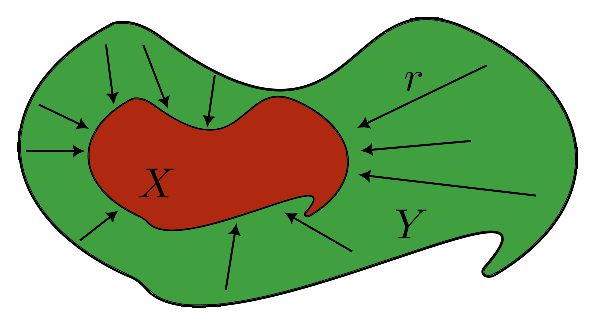
\includegraphics[scale=1.0]{Figures/retract_diagram.eps}
    \caption{Un retracci\'on $r:Y \rightarrow X$ de un espacio $Y$ hac\'ia un
    espacio  $X$.}
    \label{fig_3}
\end{figure}

Ahora recuerda que las mapas de inclusi\'on y identidad para espacios
topol\'ogicos son las mapas $i:X \rightarrow Y$ (donde $X$ es subespacio de
$Y$), y $1_X:X \rightarrow X$ dado por $i:x \rightarrow x$ y $1_X:x \rightarrow
x$ para todo $x \in X$. La definici\'on del retracto entonces se puede ver en la
siguiente diagrama, llamado una diagrama ``commutativa'':
\[\begin{tikzcd}
	&& Y \\
	\\
	\\
	X &&&& X
	\arrow["i", from=4-1, to=1-3]
	\arrow["{1_X}"', from=4-1, to=4-5]
	\arrow["r", dashed, from=1-3, to=4-5]
\end{tikzcd}\]
Entonces, seg\'un esta diagrama, $r \circ i=1_X$.

Dado una diagrama commutativa en el ``universo`` de espacios topologicos,
entonces queremos que las mapas sean mapas continuas. En este ejemplo, existe
una ``meta funci\'on`` llamado un ``functor'' $\Fc$ que lleva las espacios
topologicos hacia grupos Abelianos, tal que las diagramas commutativas son
preservada; es decir,  $\Fc$ lleva mapas continuas hacia homomorfismos.

 \begin{figure}[h]
    \centering
\[\begin{tikzcd}
	A &&&& B \\
	\\
	\\
	\\
	C
	\arrow["f", from=5-1, to=1-1]
	\arrow["g", from=1-1, to=1-5]
	\arrow["h"', from=5-1, to=1-5]
\end{tikzcd}\]
    \caption{Una diagrama commutativa, donde $A$, $B$,  $C$ son conjuntos
    cualquieras, y $f$,  $g$, y  $h$ son funciones cualquieras doned  $f \circ
g=h$.}
    \label{fig_4}
\end{figure}

\begin{lemma}\label{lemma_2.2}
    S\'i $n \geq 0$, entonces  $S^n$ no es un retracto de  $D^{n+1}$.
\end{lemma}
\begin{proof}
    Para $n=0$, es facil ver. Si  $r:D^1 \rightarrow S^0$ es un retracto,
    entonces la siguente diagrama
    \[\begin{tikzcd}
	&& {D^1} \\
	\\
	\\
	{S^0} &&&& {S^0}
	\arrow["i", from=4-1, to=1-3]
	\arrow["{1_{S^0}}"', from=4-1, to=4-5]
	\arrow["r", dashed, from=1-3, to=4-5]
\end{tikzcd}\]
nos da $r \circ i=1_{S^0}$ lo cual es imposible, ya que $S^0$ no es con\'exo, y
la imagen de  $D^1$ como subsepacio de  $S^0$ si lo es; es decir que
$r(D^1)=\{1\}$, \'o $r(D^1)=\{-1\}$. Entonces $r$ no puede ser  1--1 y sobre lo
cual contradice que  $r \circ i=1_{S^0}$ sea 1--1 y sobre.

Ahora, toma $n>0$, entonces suponga que exista una retracci\'on  $r:D^{n+1}
\rightarrow S^n$, con su diagrama de espacios topologicos y mapas continuas.
\[\begin{tikzcd}
	&& {D^{n+}} &&&&&& {H_n(D^{n+1})} \\
	\\
	\\
	{S^n} &&&& {S^n} && {H_n(S^n)} &&&& {H_n(S^n)}
	\arrow["i", from=4-1, to=1-3]
	\arrow["r", from=1-3, to=4-5]
	\arrow["{1_{S^n}}"', from=4-1, to=4-5]
	\arrow["{H_n(i)}", from=4-7, to=1-9]
	\arrow["{H_n(r)}", from=1-9, to=4-11]
	\arrow["{H_n(1_{S^n})}"', from=4-7, to=4-11]
\end{tikzcd}\]
Entonces $r \circ i=1_{s^n}$. Aplicando un functor particular llamado $H_n$,
obtemeos una diagrama commutativa de grupos Abelianos y homomorfismos. Las dos
diagramas se pueden ver arriba. Entonces tenemos que $H_n(S^n)=\Z$, y
$H_n(D^{n+1})=\vbrack{0}$. Ahora tenemos que $H_n(r) \circ
H_n(i)=H_n(1_{S^n})=1_\Z$. Esto es imposible ya que $1_\Z$ no se facotriza sobre
$\vbrack{0}$; i.e. $H_n(r) \circ H_n(i)=0 \ne 1_\Z$. Por lo tanto $S^n$ no
puede ser un retracto de  $D^{n+1}$.
\[\begin{tikzcd}
	&& \langle0\rangle \\
	\\
	\\
	\Z &&&& \Z
	\arrow["{H_n(i)}", from=4-1, to=1-3]
	\arrow["{H_n(r)}", from=1-3, to=4-5]
	\arrow["{1_\Z}"', from=4-1, to=4-5]
\end{tikzcd}\]
\end{proof}

Ahora reiteremos la teorema de Brouwer para la demostraci\'on para $n$ general.

\begin{theorem}[Teorema de Puntos Fijos de Brouwer]
    S\'i $f:D^n \rightarrow D^n$ es una funci\'on continua, entonces existe un
    punto fijo en $D^n$ para toda $n \geq 1$.
\end{theorem}
\begin{proof}
    Para $n>1$, suponga que no hay puntos fijos. Entonces sea $f:D^n \rightarrow
    D^n$ y que $f(x) \neq x$ para todo $x \in D^n$. Defina entonces, la mapa
    $g:D^n \rightarrow S^{n-1}$ dado por la figura \ref{fig_5}.
    \begin{figure}[h]
        \centering
        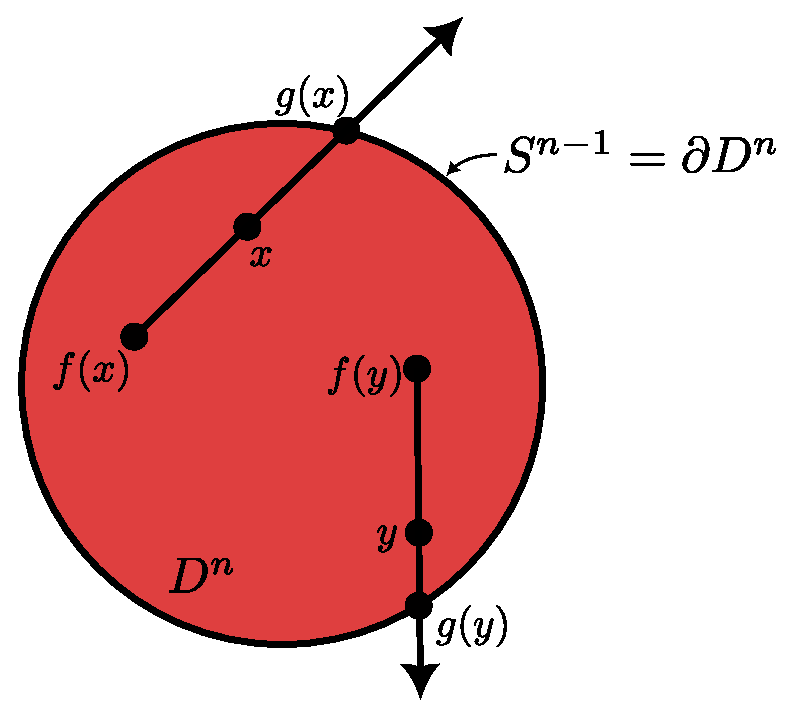
\includegraphics[scale=0.5]{Figures/brouwer_thm_2.eps}
        \caption{}
        \label{fig_5}
    \end{figure}
    Note que $g$ es continua, y que  $g(x)=x$ para todo $x \in S^{n-1}$. Puse,
    vemos que $g$ es una retracci\'on, lo cual es imposible por el lema
    \ref{lemma_2.2} Por lo tanto, no existen puntos fijos.
\end{proof}

\section*{Lectura 3: Categor\'ias y Funtores.}

\begin{definition}
    Definimos una \textbf{clase} de ser una colecci\'on de objetos tal que s\'i
    $T$ y  $A$ son clases, entonces  $A \notin T$.
\end{definition}

\begin{definition}
    Una \textbf{categor\'ia} $\Cc$ es un clase de objetos denotados por
    $\obj{\Cc}$ junto a una colecci\'on de conjuntos $\Hom{(X,Y)}$,  para
    cualquieras $X,Y \in \obj{\Cc}$, de \textbf{morfismos} de $X$ hac\'ia $Y$,
    cuyas elementos estan denotados $f:X \rightarrow Y$ \'o $X \xrightarrow{f}
    Y$, y una operac\i\'on binaria $\circ:\Hom{(X,Y)} \times \Hom{(Y,Z)}
    \rightarrow \Hom{(X,Z)}$ llamado \textbf{composici\'on} tal que si $f:X
    \rightarrow Y$ y $g:Y \rightarrow Z$ son morfismos, entonces $g \circ f:X
    \rightarrow Z$ es un morfismo y:
    \begin{enumerate}
        \item[(1)] $\Hom{(X,Y)}$ y $\Hom{(A,B)}$ son disjuntas.

        \item[(2)] La composici\'on $\circ$ es associativa s\'i esta definido.
            Es decir, sy  $g \circ (f \circ h)$ \'o $(g \circ g) \circ h$
            existen en $\Hom{(X,Y)}$, entonces $g \circ (f \circ h)=(g \circ f)
            \circ g$.

        \item[(3)] $\Hom{(X,X)}$ no es vac\'io y existe al menos un morfismo
            $1_X:X \rightarrow X$, llamado la \textbf{identidad} de $X$, tal que
            $1_X \circ f=f$ y  $g \circ 1_X=g$ para morfismos  $f:X \rightarrow
            Y$ y $g:Z \rightarrow X$, para cualquieras objetos $X,Y,Z \in
            \obj{\Cc}$
    \end{enumerate}
\end{definition}

\begin{definition}
    Sea $\Cc$ una categor\'ia. Se llama el conjunto $\Mc_\Cc$  \textbf{los
    morfismos de la categor\'ia} donde $\Mc_\Cc$ es la union de todos los
    conjuntos $\Hom{(X,Y)}$ para todos $X,Y \in \obj{\Cc}$.
\end{definition}

\begin{figure}[h]
    \centering
    \[\begin{tikzcd}
	X &&& Y &&& Z
	\arrow["f", from=1-1, to=1-4]
	\arrow["g", from=1-4, to=1-7]
	\arrow["{g \circ f}"', curve={height=30pt}, from=1-1, to=1-7]
\end{tikzcd}\]
    \caption{Un ejemplo de composici\'on de morfismos de una categor\'ia}
    \label{fig_6}
\end{figure}

\begin{figure}[h]
    \centering
    \[\begin{tikzcd}
	X & X &&& Y & Y
	\arrow[curve={height=12pt}, from=1-2, to=1-5]
	\arrow[curve={height=-12pt}, from=1-2, to=1-5]
	\arrow[from=1-2, to=1-5]
	\arrow["{1_X}", from=1-2, to=1-1]
	\arrow["{1_Y}", from=1-5, to=1-6]
	\arrow[curve={height=24pt}, from=1-5, to=1-2]
	\arrow[curve={height=-24pt}, from=1-5, to=1-2]
\end{tikzcd}\]
    \caption{Morfismos entre dos objetos $X$ y  $Y$ de una categor\'ia
    incluyendo las identidades de $X$ y $Y$}
    \label{fig_7}
\end{figure}

\begin{example}\label{}
    \begin{enumerate}
        \item[(1)] Considere la categor\'ia $\Cc=\Conj$, donde  $\boj{\Cc}$ es
            la clase de todo los conjuntos. Los morfismos de $\Cc$ son
            funci\'ones  $f:X \xrightarrow{} Y$ de un conjunto $X$ hac\'ia un
            conjunto  $Y$.

        \item[(2)] Sea $\Cc=\Top$ la categor\'ia de espacios topol\'ogicos,
            donde  $\obj{\Cc}$ es la colecci\'on de todas las espacios
            topol\'ogicos. Los morfismos de $\Top$ son funci\'ones continuas
            entre espacios topologicos. Es decir, $\Hom{(X,Y)}=\{f : f:X
            \xrightarrow{} Y \text{ es continua}\}$. La composici\'on de
            morfismos es la composicion de funciones usual.

        \item[(3)] Sea $\Cc=\Grp$ la categor\'ia de grupos, cuyas objetos son
            todo los grupos. Entonces los morfismos de  $\Grp$ estan definido
            por los conjuntos  $\Hom{(G,H)}=\{\phi : \phi:G \xrightarrow{} H
            \text{ es un homomrfismo}\}$. La composici\'on de morfismos es la
            composicion de funciones usual.
    \end{enumerate}
\end{example}

\begin{definition}
    Sean $\Cc$ y  $\Ac$ categor\'ias con  $\obj{\Cc} \subseteq \obj{\Ac}$.
    Decimos que $\Cc$ es una \textbf{subcategor\'ia} de $\Ac$ s\'i
    $\Hom_\Cc{(X,Y)} \subseteq \Hom_\Ac{(X,Y)}$ para todo $X,Y \in \obj{\Cc}$ ty
    la composici\'on de $\Cc$ es la misma de  $\Ac$.
\end{definition}

\begin{example}\label{}
    \begin{enumerate}
        \item[(1)] Tenemos que $\Top$ y  $\Grp$ son subcategor\'ias de
            $\Conj$.
        \item[(2)] La categor\'ia $\Top^2$ de pares topologicos tiene como objetos
            son todas pares  $(X,A)$, donde $X$ es un espacio topol\'ogico y $A
            \subseteq X$ es subsepacio de $X$. Los morfismos de $\Top^2$, para
            pare topologicos  $(X,Y)$ y $(Y,B)$, son las funciones continuas
            $f:X \xrightarrow{} Y$ donde $f(A) \subseteq B$ es subespacio de $B$.

        \item[(3)] La categor\'ia $\Top^*$ de pares topologicos  $(X,a)$, donde
            $a$ es un punto en  $X$ es una subcategor\'ia de  $\Top^2$.
    \end{enumerate}
\end{example}

\begin{definition}
    Sea $\Cc$ una categor\'ia. Una \textbf{diagrama} de objetos y morfismos en
    $\Cc$ es un grafo dirigido cuya cunjunto de vertices es subconjunto de
    $\obj{\Cc}$ y cuyas aristas son morfismos entre esos vertices. Decimos que
    una diagrama es \textbf{commutativo} si para cualquieras vertices $A,B,C,D$
    en la diagrama, y cualquier morfismos  $f:A \xrightarrow{} B$, $i:C
    \xrightarrow{} D$, $h:A \xrightarrow{} C$, y $g:B \xrightarrow{} D$, tenemos
    que $g \circ f=i \circ h$.
\end{definition}

\begin{example}\label{}
    Las figuras \ref{fig_6} y \ref{fig_7} son ejemplos de diagramas de objetos y
    morfismos en una categori\'ia.
\end{example}

\begin{figure}[h]
    \centering
    \[\begin{tikzcd}
	A &&&&& B \\
	\\
	\\
	C &&&&& D
	\arrow["f", from=1-1, to=1-6]
	\arrow["i", from=4-1, to=4-6]
	\arrow["g", from=1-6, to=4-6]
	\arrow["h"', from=1-1, to=4-1]
	\arrow["{g \circ f=i \circ h}", dashed, from=1-1, to=4-6]
\end{tikzcd}\]
    \caption{Un diagrama commutativa entre objetos y morfismos de una
    categor\'ia.}
    \label{fig_8}
\end{figure}

%\section*{Lectura 3: Categor\'ias y Funtores.}

%\section*{Lectura 5: Teoremas de Isomorfismo.}

\[\begin{tikzcd}
	& {\faktor{\Z}{24\Z}} &&&&&& \Z \\
	{\langle 2 \rangle} && {\lang 3 \rang} && 2\Z & 3\Z & 5\Z & 7\Z & \dots \\
	{\lang 4 \rang} && {\lang 6 \rangle} && 4\Z & 6\Z & 9\Z & 10\Z & \dots \\
	{\langle 8 \rangle} && \langle12\rangle && 8\Z & 12\Z & 18\Z & 20\Z & \dots \\
	& {\langle 0 \rangle} &&& \vdots & 24\Z & \vdots & \vdots & \dots
	\arrow[no head, from=1-2, to=2-1]
	\arrow[no head, from=2-1, to=3-1]
	\arrow[no head, from=3-1, to=4-1]
	\arrow[no head, from=4-1, to=5-2]
	\arrow[no head, from=5-2, to=4-3]
	\arrow[no head, from=4-3, to=3-1]
	\arrow[no head, from=4-3, to=3-3]
	\arrow[no head, from=3-3, to=2-3]
	\arrow[no head, from=2-3, to=1-2]
	\arrow[no head, from=2-1, to=3-3]
	\arrow[no head, from=1-8, to=2-5]
	\arrow[no head, from=1-8, to=2-6]
	\arrow[no head, from=1-8, to=2-7]
	\arrow[no head, from=1-8, to=2-8]
	\arrow[no head, from=1-8, to=2-9]
	\arrow[no head, from=2-5, to=3-5]
	\arrow[no head, from=2-5, to=3-6]
	\arrow[no head, from=2-5, to=3-8]
	\arrow[no head, from=2-5, to=3-9]
	\arrow[no head, from=2-6, to=3-6]
	\arrow[no head, from=2-6, to=3-7]
	\arrow[no head, from=2-6, to=3-9]
	\arrow[no head, from=3-5, to=4-5]
	\arrow[no head, from=3-5, to=4-6]
	\arrow[no head, from=3-5, to=4-8]
	\arrow[no head, from=3-5, to=4-9]
	\arrow[no head, from=4-5, to=5-5]
	\arrow[no head, from=4-7, to=5-8]
	\arrow[no head, from=4-7, to=5-9]
	\arrow[no head, from=4-6, to=5-6]
	\arrow[no head, from=4-5, to=5-6]
	\arrow[no head, from=4-6, to=5-8]
	\arrow[no head, from=4-7, to=5-7]
	\arrow[no head, from=3-6, to=4-6]
	\arrow[no head, from=3-6, to=4-8]
	\arrow[no head, from=3-6, to=4-9]
	\arrow[no head, from=4-6, to=5-9]
\end{tikzcd}\]

\[\begin{tikzcd}
	& \Z \\
	2\Z && 3\Z \\
	4\Z && 6\Z \\
	8\Z && 12\Z \\
	& 24\Z
	\arrow[no head, from=1-2, to=2-1]
	\arrow[no head, from=2-1, to=3-3]
	\arrow[no head, from=3-3, to=4-3]
	\arrow[no head, from=4-3, to=3-1]
	\arrow[no head, from=3-1, to=4-1]
	\arrow[no head, from=4-1, to=5-2]
	\arrow[no head, from=5-2, to=4-3]
	\arrow[no head, from=3-3, to=2-3]
	\arrow[no head, from=2-3, to=1-2]
	\arrow[no head, from=2-1, to=3-1]
\end{tikzcd}\]

%\section*{Lectura 6: La Teoreman Fundamental del Algebra.}

\begin{theorem}[La Teorema Fundamental del Algebra]\label{thm_6.11}
    Todo polinomio con coeficientes complejas tiene al menos una ra\'iz
    complejo.
\end{theorem}
\begin{proof}
    Sea $\Sigma_\rho \subseteq \C$ el circulo de radio  $\rho$ en  $\C$.
    Considere la mapa  $f:\C \xrightarrow{} \C$ dado por $f(z)=z^n$, y denota
    $f^n_\rho=f|_{\Sigma_\rho}$. Nota que los $f^n_\rho$ son homotopicamentes
    nulas.

    Ahora, considere el polinomio  $g(z)=z^n+a_{n-1}z^{n-1}+\dots+a_1z+a_0$
    donde $a_i \in \C$ para todo  $0 \leq i \leq n$ y  $\deg{g}=n \geq 1$.
    Escoga $\rho>\max{\{1,\sum{|a_i|}\}}$, y defina la mapa $F:\Sigma_\rho
    \times I \xrightarrow{} \C$ dado por
    \begin{equation*}
        F(z,t)=z^n+\sum_{i=0}^{n-1}{(1-t)a_iz^i}
    \end{equation*}
    Por la contunuidad de polinomios en $\C$, tenemos que  $F$ es continua. Mas
    a\'un tenemos que  $F(z,0)=z^n+a_{n-1}z^{n-1}+\dots+a_1z_1+a_0=g(z)$ y
    $F(z,1)=z^n=f^n_\rho$. As\'i que $f^n_\rho \simeq g$ son homotopicos atraves
    de la homotopia $F$.

    Afirmamos que $F(z,t) \neq 0$. Por lo contrario, asuma que existe un $(z,t)
    \in \Sigma_\rho \times I$ tal que $F(z,t)=0$. Entonces tenemos que
    \begin{equation*}
        z^n=-\sum_{i=0}^{n-1}{(1-t)a_iz^i}
    \end{equation*}
    Por la desigualdad de triangulo, tenemos
    \begin{equation*}
        |z^n|=\rho^n \leq \sum{(1-t)|a_i|\rho^i} \leq \rho^{n-1}\sum{(1-t)|a_i|}
    \end{equation*}
    como $\rho>1$ y  $t \in I$ implica que  $\sum{(1-t)|a_i|} \leq \sum{|a_|}$,
    tenemos que
    \begin{equation*}
        \rho \leq \sum_{i=0}^{n-1}{(1-t)|a_i|}
    \end{equation*}
    lo cual contradice neustor escojido de $\rho$. Asi que  $F(z,t) \neq 0$ para
    todos $(z,t) \in \Sigma_\rho \times I$.

    \begin{figure}[h]
        \centering
        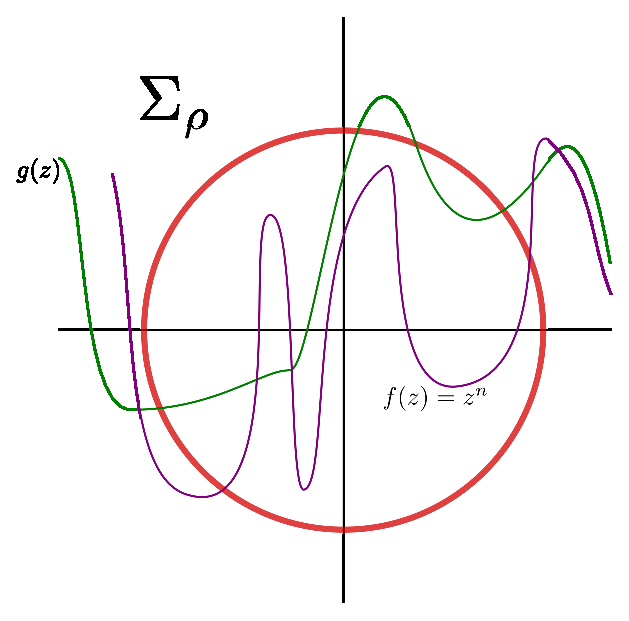
\includegraphics[scale=0.5]{Figures/fund_thm_algebra.eps}
        \caption{La teorema Fundamental del Algebra. Nota que $f^n_\rho$ consiste de
        cuyas puntos de $f(z)=z^n$ cuyas puntos intersecan con $\Sigma_\rho$.}
        \label{fig_16}
    \end{figure}

    Finalmente, tenemos que $F:\Sigma_\rho \times I \xrightarrow{}
    \com{\C}{\{0\}}$. Entonces suponga que $g(z)$ no tiene raices complejas.
    Defina $G:\Sigma_\rho \times I \xrightarrow{} \com{\C}{\{0\}}$ dado por
    $G(z,t)=g((1-t)z)$. Tenemos que $(1-t)z$ es una mapa continua, y que $g$ es
    continua; por lo tanto por composici\'on,  $G$ tambien es continua  (de
    hecho, es continua en $z$ y en  $t$). Mas a\'un, tenemos $G(z,0)=g(z)$ y
    $G(z,1)=g(0)=a_0$. As\'i que $g$ es homotopica a la mapa constante  $k:z
    \xrightarrow{} a_0$, por lo tanto es homotopicamente nula. Por transitividad
    de homotopia, $f^n_\rho$ tambien es homotopicamente nula, lo cual es
    imposible. Por lo tanto,  $g$ tiene que tener al menos una raiz en $\C$.
\end{proof}

\end{document}
